%-------------------------------------------------------------------------------
% RESULTS AND DISCUSSION
%-------------------------------------------------------------------------------

\section{Results} \label{sec:resdisc}

The fist goal is to reproduce the bifurcation diagram in figure
\ref{bif_diag_chen} now using the regularized version. The regularized
bifurcation diagram is shown below and a list of bifurcations occurred in the
regularized version and their exact locations. The locations of the have been
obtained by linearly interpolating the eigenvalues between two states obtained
by the pseudo-archlength continuation.

\begin{table}[h!]
  \caption{List of bifurcations encountered and the critical $\Rey$ at which they
    occur}
  \label{tab:bif_points}
\begin{tabular}{l c}
Bifurcation & $\Rey$\\
\hline
$P_1$, first supercritical pitchfork of the base flow & \\
$P_2$, second pitchfork of the base flow & \\
$SN$, saddle-node bifurcation of the asymmetric steady solution&  \\
$H$, Hopf bifurcation of the asymmetric steady solution&  \\
\end{tabular}
\end{table}

\begin{table}[h!]
  \caption{Critical Reynolds numbers of the two
    pitchfork bifurcations of the symmetric base flow, $\Rey_c^{P_1}$
    and $\Rey_c^{P_2}$, and of the saddle-node and Hopf bifurcations
    corresponding to the asymmetric steady solution, $\Rey_c^{H}$ and
    $\Rey_c^{SN}$, respectively. For the Hopf bifurcation, the imaginary part
    $\omega_c^{H}$ corresponding to the crossing eigenvalue has also been
    included.}
  \label{tab:re_crit}
\begin{tabular}{crrrrrr}
$M$ & $\Rey_c^{P_1}$ & $\Rey_c^{P_2}$ & $\Rey_c^{H}$ &  $\omega_c^{H}$ & $\Rey_c^{SN}$  \\
\hline
$48$ &  & &          &          &   \\
$64$ &  & &          &          &   \\
$96$ &  & &          &          &   \\
\end{tabular}
\end{table}

\begin{figure}[h!]
  \begin{center}
  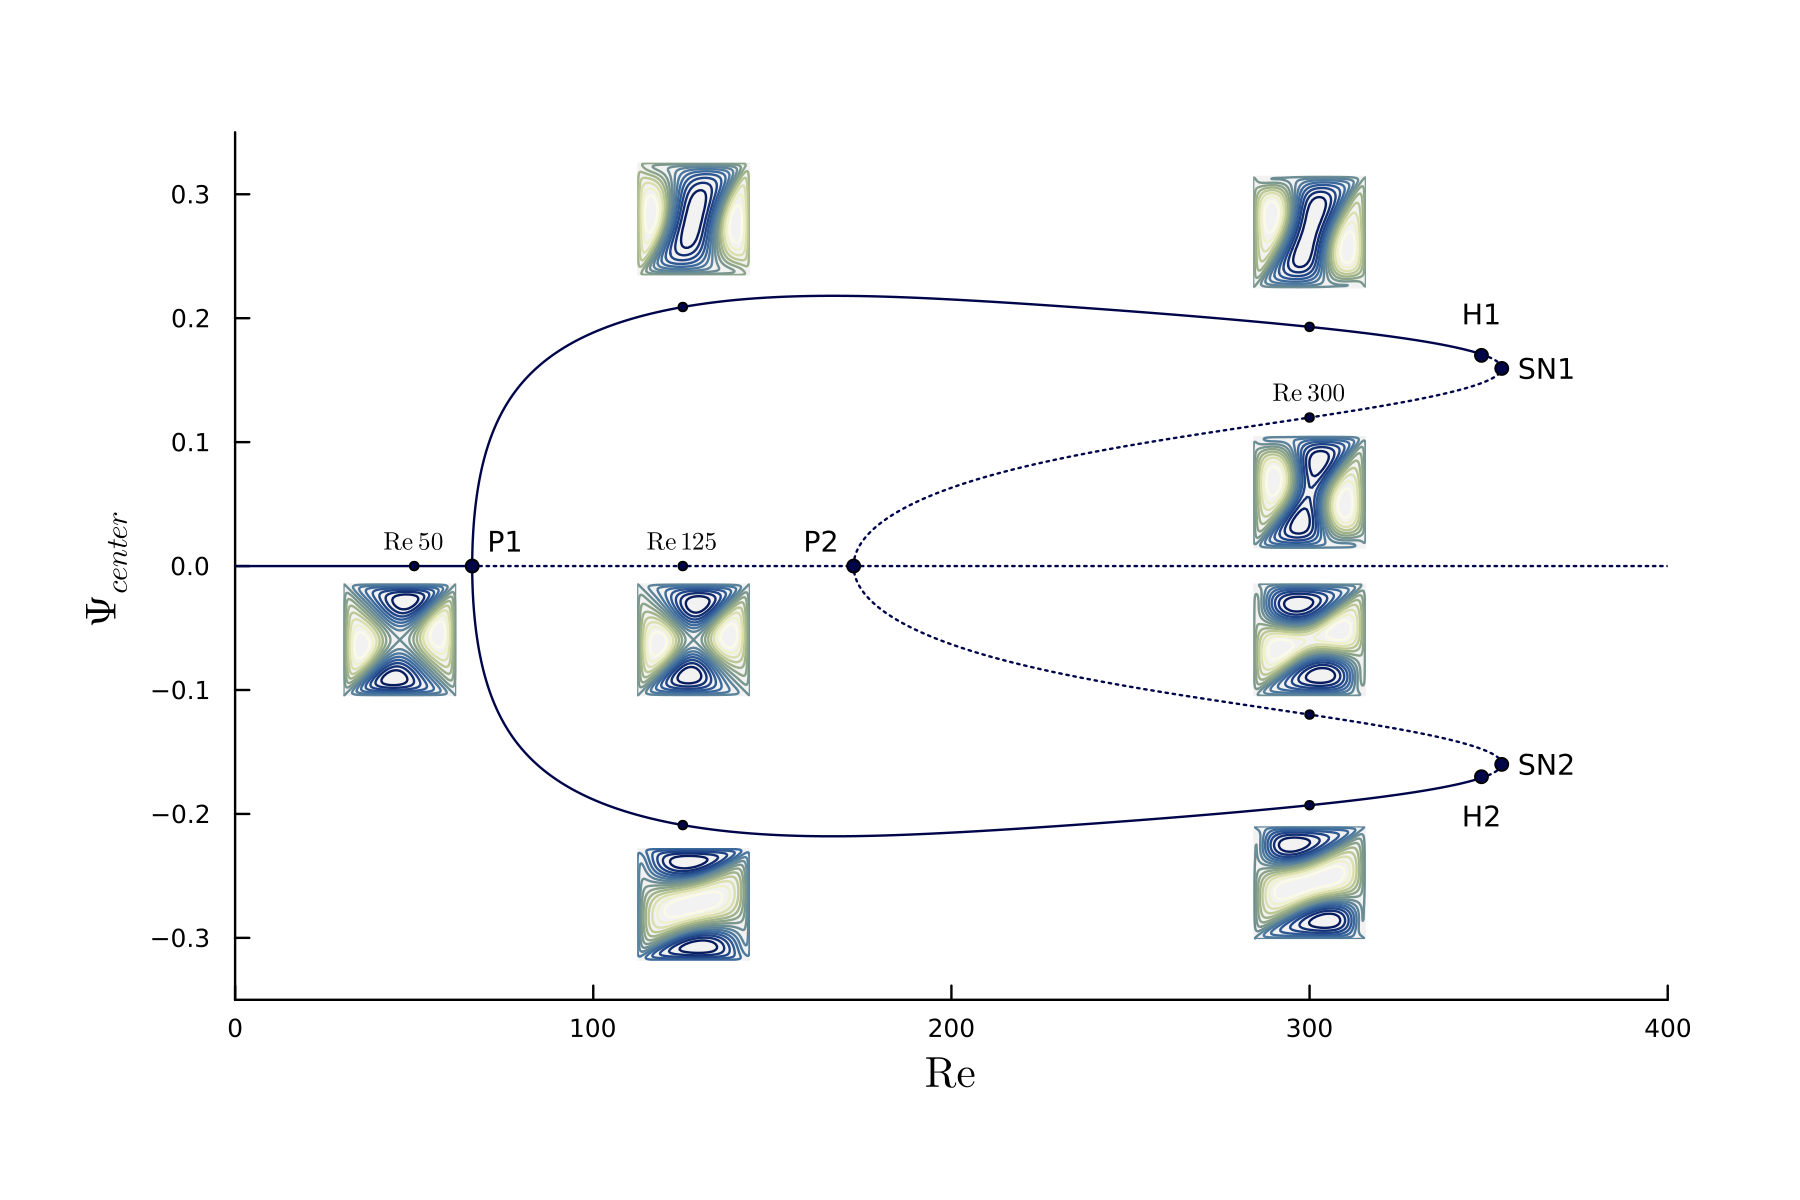
\includegraphics[width=\textwidth]{figs/bifurcation_diag64x64.png}
  \end{center}
  \label{fig:bif_diag}
  \caption{Bifurcation diagram for the regularized version of the four-sided
    cavity flow, calculated with the developed Julia package} 
\end{figure}

First of all on can see that the bifurcation diagram regularized version
resembles the non-regularized version. The reported critical Reynolds numbers
for the pitchfork 2 seem to be close. One can also see how the regularized
version is converging very quickly, only the third digits are changing from a
grid of 48x48 onwards for the two pitchforks. On has to as well note that the
pitchfork 2 is not actually a pitchfork as only unstable branches (denoted by
the dashed line) join.   

On the contrary the saddle-node is quite far off the original value by around
100 in Reynolds. It has been found that increasing the ( will move the
saddle-node more to the right. 

Furthermore a Hopf bifurcation at around $348$ has been found. This was not
reported in any of the previous studies. The question which arises is if the
Hopf bifurcation is sub-critical or super-critical. Launching the time-stepper
slightly after the Hopf will give a stable periodic orbit. This is shown in
figure \ref{fig:orbit}. To visualize the orbit the phase space is    

\begin{figure}[h!]
  \begin{center}
  \includegraphics[width=0.6*\textwidth]{figs/orbits}
  \end{center}
  \label{fig:orbit}
  \caption{Periodic orbits in function of the midpoints} 
\end{figure}

\begin{figure}[h!]
  \begin{center}
  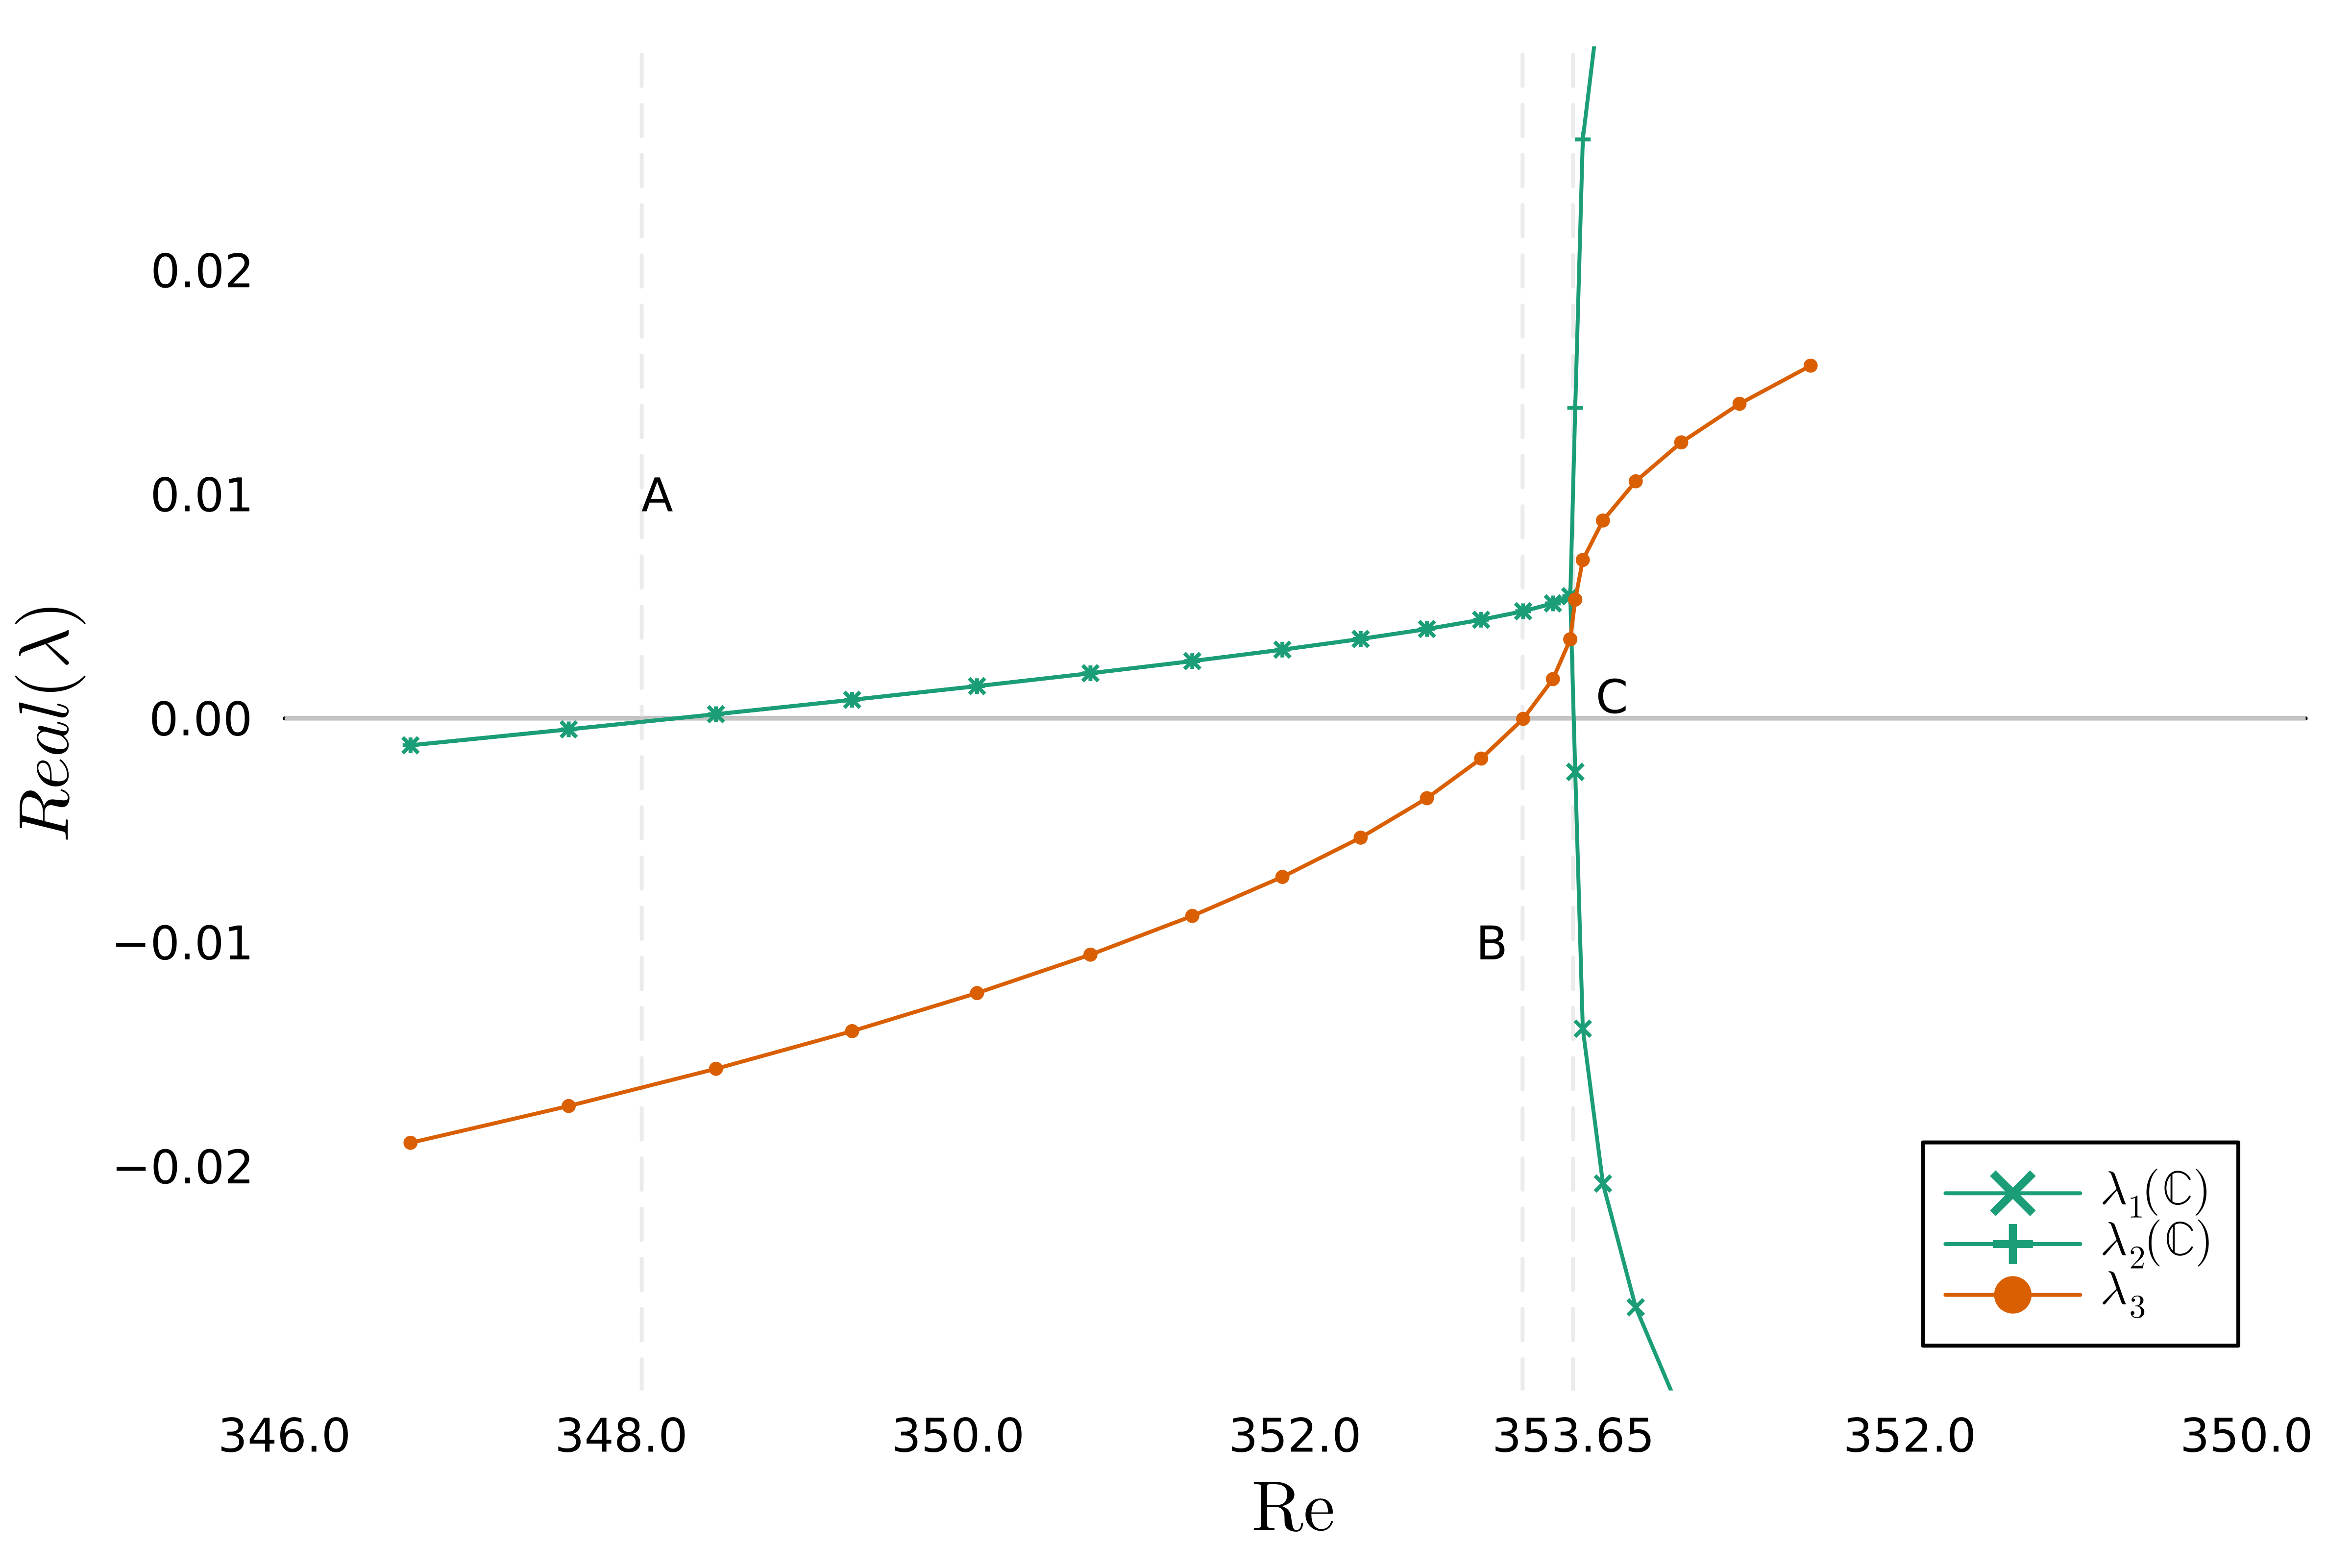
\includegraphics[width=0.6*\textwidth]{figs/lsa_sn}
  \end{center}
  \label{fig:lsa}
  \caption{Linear stability analysis around saddle node (increasing and the decreasing Renolds number). The real
    part of the largest eigenvalues are plotted} 
\end{figure}


The linear stability analysis around the saddle node shows firstly the crossing
of the complex conjugate pair (in green) referred to as point A. Then there is
another crossing at 

\begin{figure}[h!]
  \begin{center}
  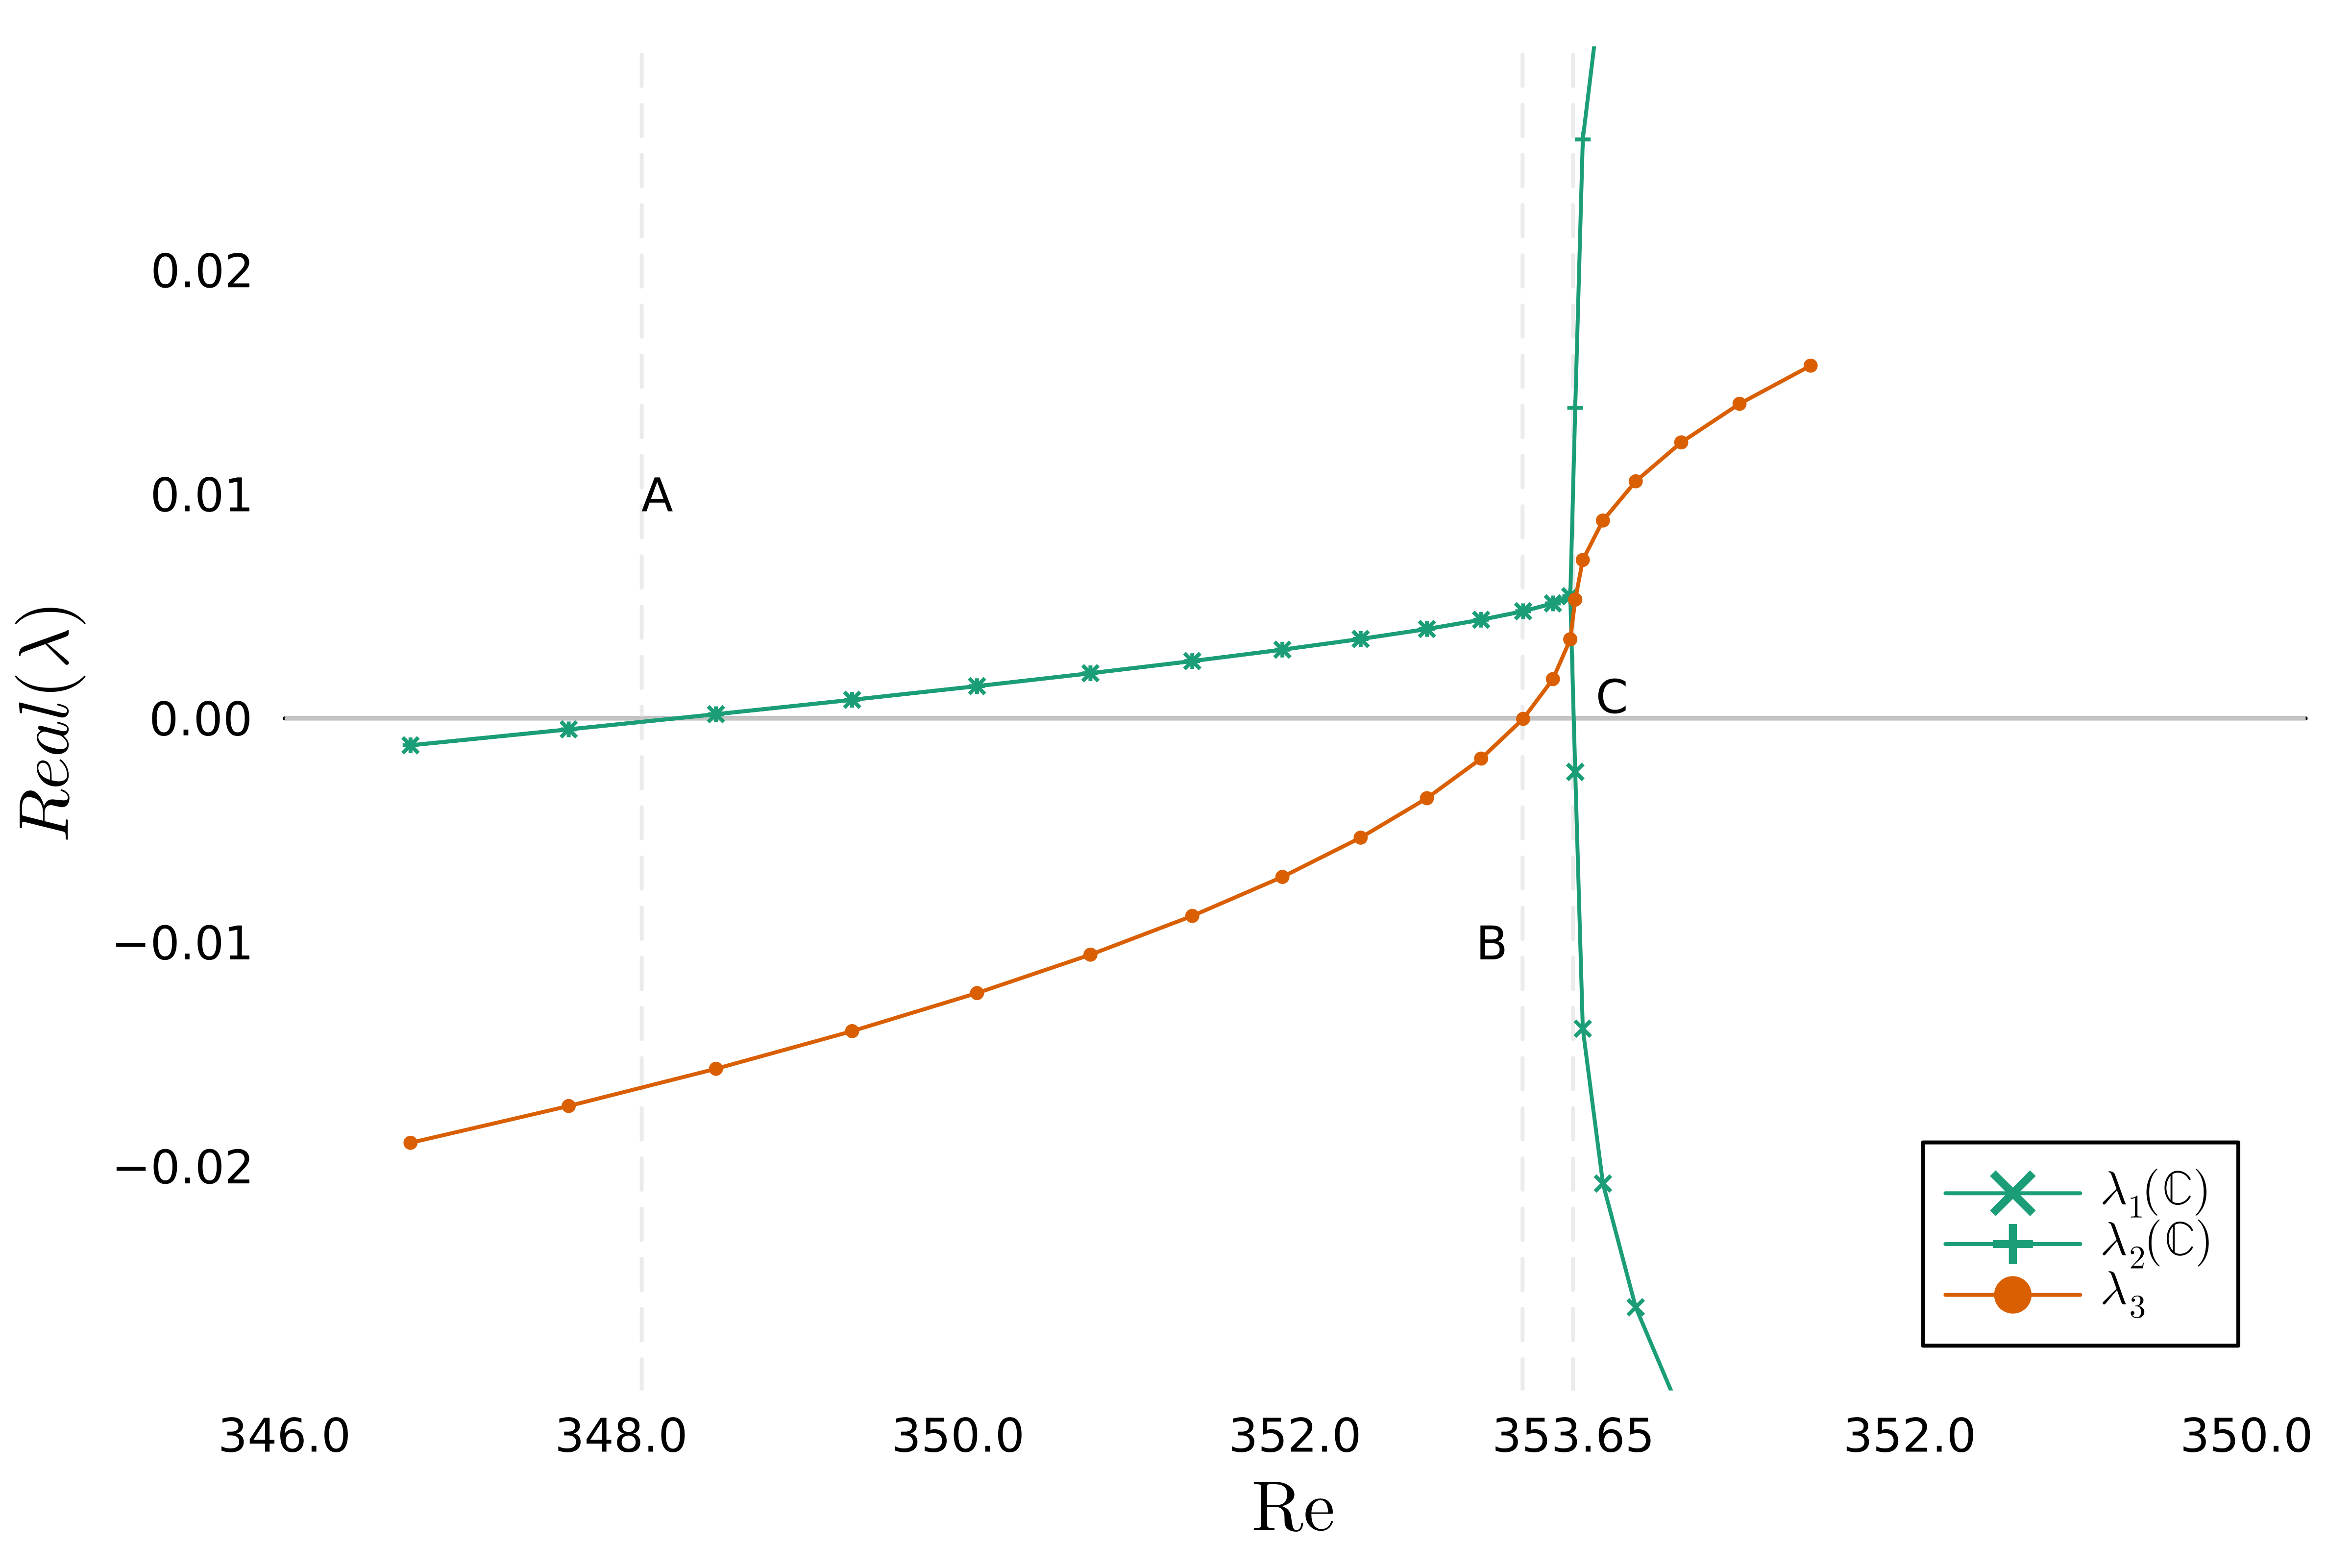
\includegraphics[width=0.6*\textwidth]{figs/lsa_sn}
  \end{center}
  \label{fig:lsa}
  \caption{Linear stability analysis around saddle node (increasing and the decreasing Renolds number). The real
    part of the largest eigenvalues are plotted} 
\end{figure}

Close to the saddle node there is another branch appearing this branch is. This
can be detected by starting natural continuation algorithm close to branch.
This branch is depicted in figure \ref{secondbranch}. And one can see how the

It
is not yet clear what actually happens there but the simplest explanation being
that at the first crossing B in figure \ref{fig:lsa} corresponds to the
emergence of this new branch. But a linear stability analysis around shows that
the linear stability analysis around the saddle node shows that the complex
conjugate pair seems to be 0 at this precise location. Below the values at the
center of the streamfunction are compared for the different eigenvalue crossing.

\begin{table}[h!]
  \caption{\Psi
    Critical Reynolds numbers of the two
    pitchfork bifurcations of the symmetric base flow, $\Rey_c^{P_1}$
    and $\Rey_c^{P_2}$, and of the saddle-node and Hopf bifurcations
    corresponding to the asymmetric steady solution, $\Rey_c^{H}$ and
    $\Rey_c^{SN}$, respectively. For the Hopf bifurcation, the imaginary part
    $\omega_c^{H}$ corresponding to the crossing eigenvalue has also been
    included.}
  \label{tab:re_crit}
\begin{tabular}{crrrrrr}
$M$ & $\Rey_c^{P_1}$ & $\Rey_c^{P_2}$ & $\Rey_c^{H}$ &  $\omega_c^{H}$ & $\Rey_c^{SN}$  \\
\hline
$48$ &  & &          &          &   \\
$64$ &  & &          &          &   \\
$96$ &  & &          &          &   \\
\end{tabular}
\end{table}

\begin{figure}[h!]
  \begin{center}
  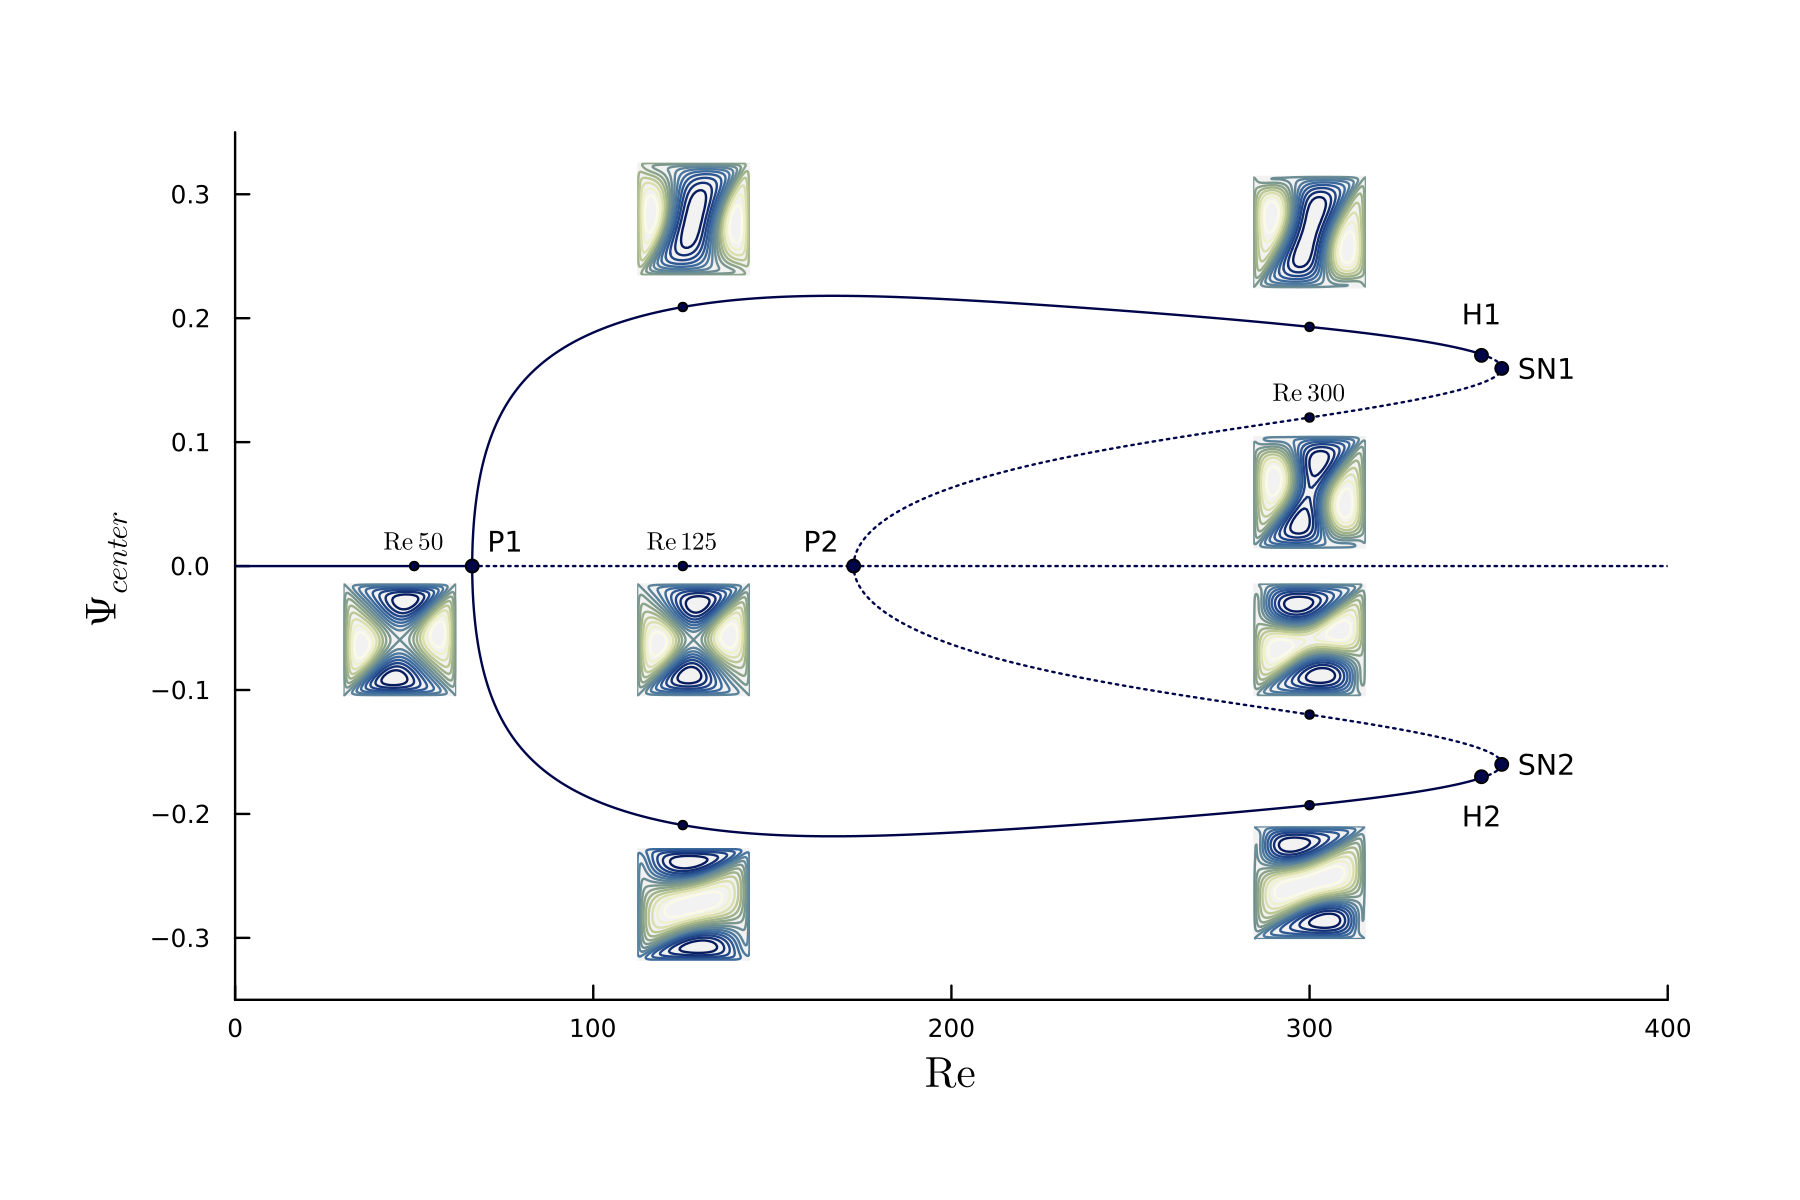
\includegraphics[width=\textwidth]{figs/bifurcation_diag64x64.png}
  \end{center}
  \label{fig:bif_diag}
  \caption{Bifurcation diagram for the regularized version of the four-sided
    cavity flow, calculated with the developed Julia package} 
\end{figure}

First of all on can see that the bifurcation diagram regularized version
resembles the non-regularized version. The reported critical Reynolds numbers
for the pitchfork 2 seem to be close. One can also see how the regularized
version is converging very quickly, only the third digits are changing from a
grid of 48x48 onwards for the two pitchforks. On has to as well note that the
pitchfork 2 is not actually a pitchfork as only unstable branches (denoted by
the dashed line) join.   

On the contrary the saddle-node is quite far off the original value by around
100 in Reynolds. It has been found that increasing the ( will move the
saddle-node more to the right. 

Furthermore a Hopf bifurcation at around $348$ has been found. This was not
reported in any of the previous studies. The question which arises is if the
Hopf bifurcation is sub-critical or super-critical. Launching the time-stepper
slightly after the Hopf will give a stable periodic orbit. This is shown in
figure \ref{fig:orbit}. To visualize the orbit the phase space is    

\begin{figure}[h!]
  \begin{center}
  \includegraphics[width=0.6*\textwidth]{figs/orbits}
  \end{center}
  \label{fig:orbit}
  \caption{Periodic orbits in function of the midpoints} 
\end{figure}

\begin{figure}[h!]
  \begin{center}
  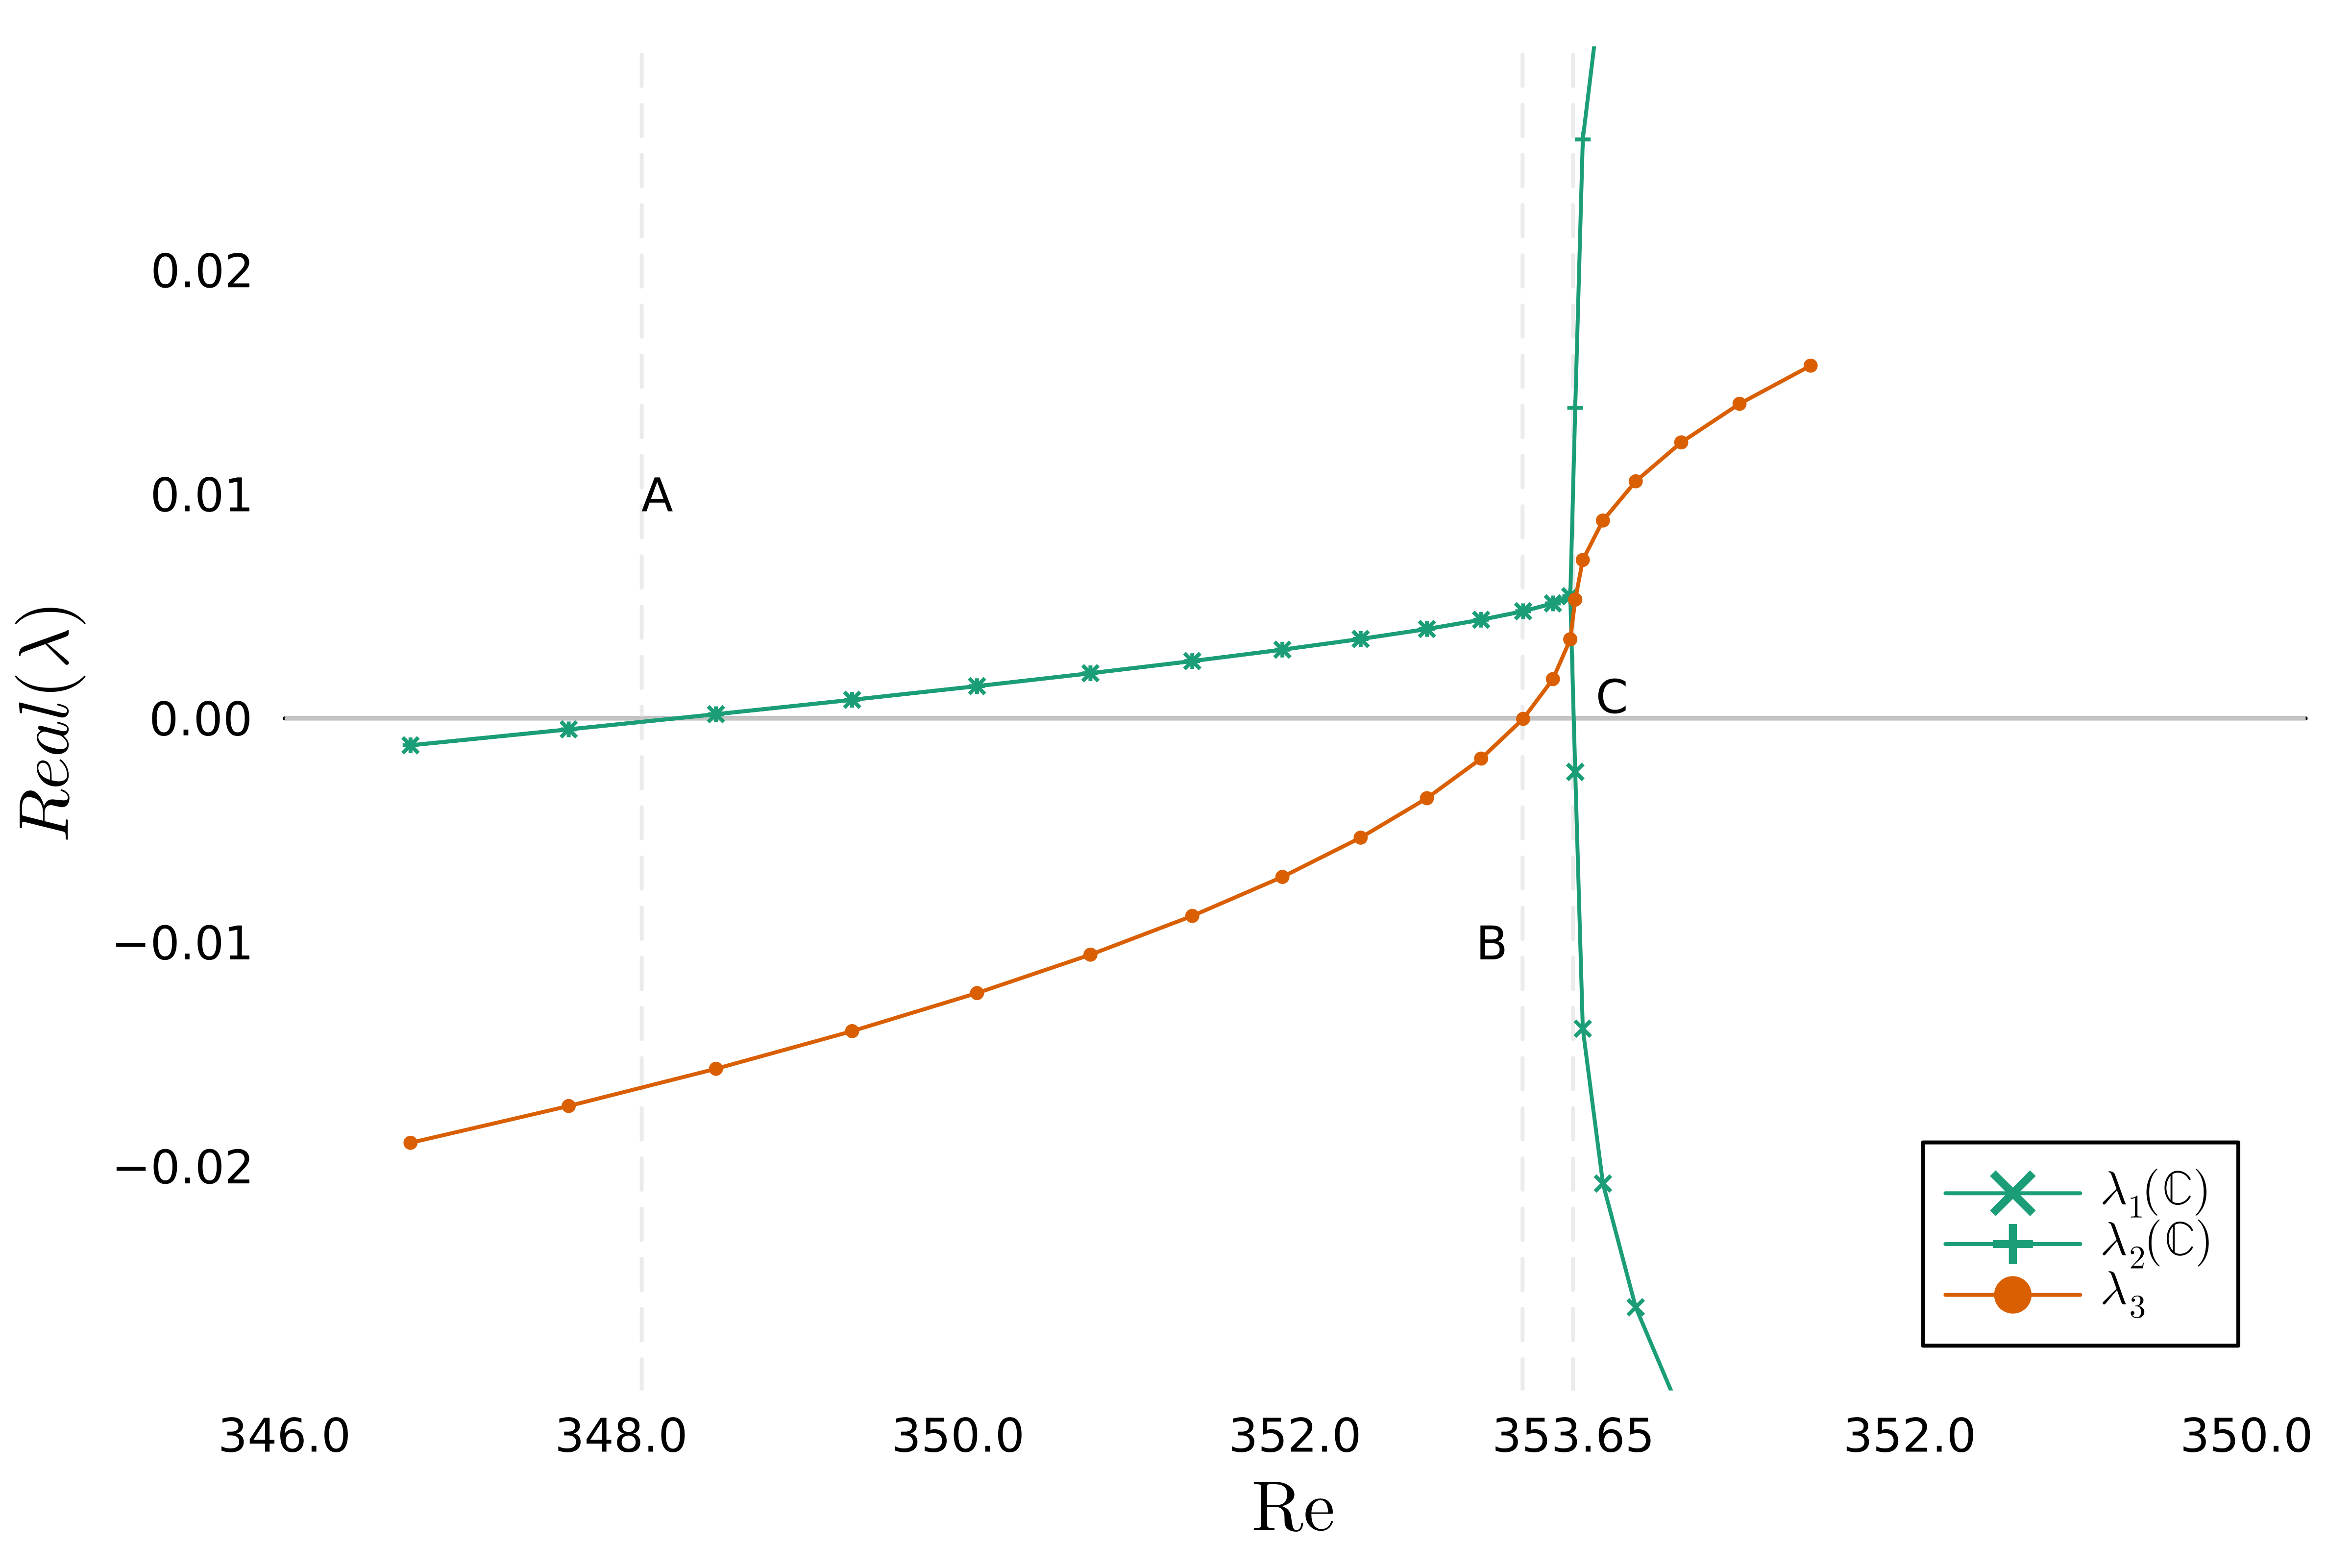
\includegraphics[width=0.6*\textwidth]{figs/lsa_sn}
  \end{center}
  \label{fig:lsa}
  \caption{Linear stability analysis around saddle node (increasing and the decreasing Renolds number). The real
    part of the largest eigenvalues are plotted} 
\end{figure}


The linear stability analysis around the saddle node shows firstly the crossing
of the complex conjugate pair (in green) referred to as point A. Then there is
another crossing at 

\begin{figure}[h!]
  \begin{center}
  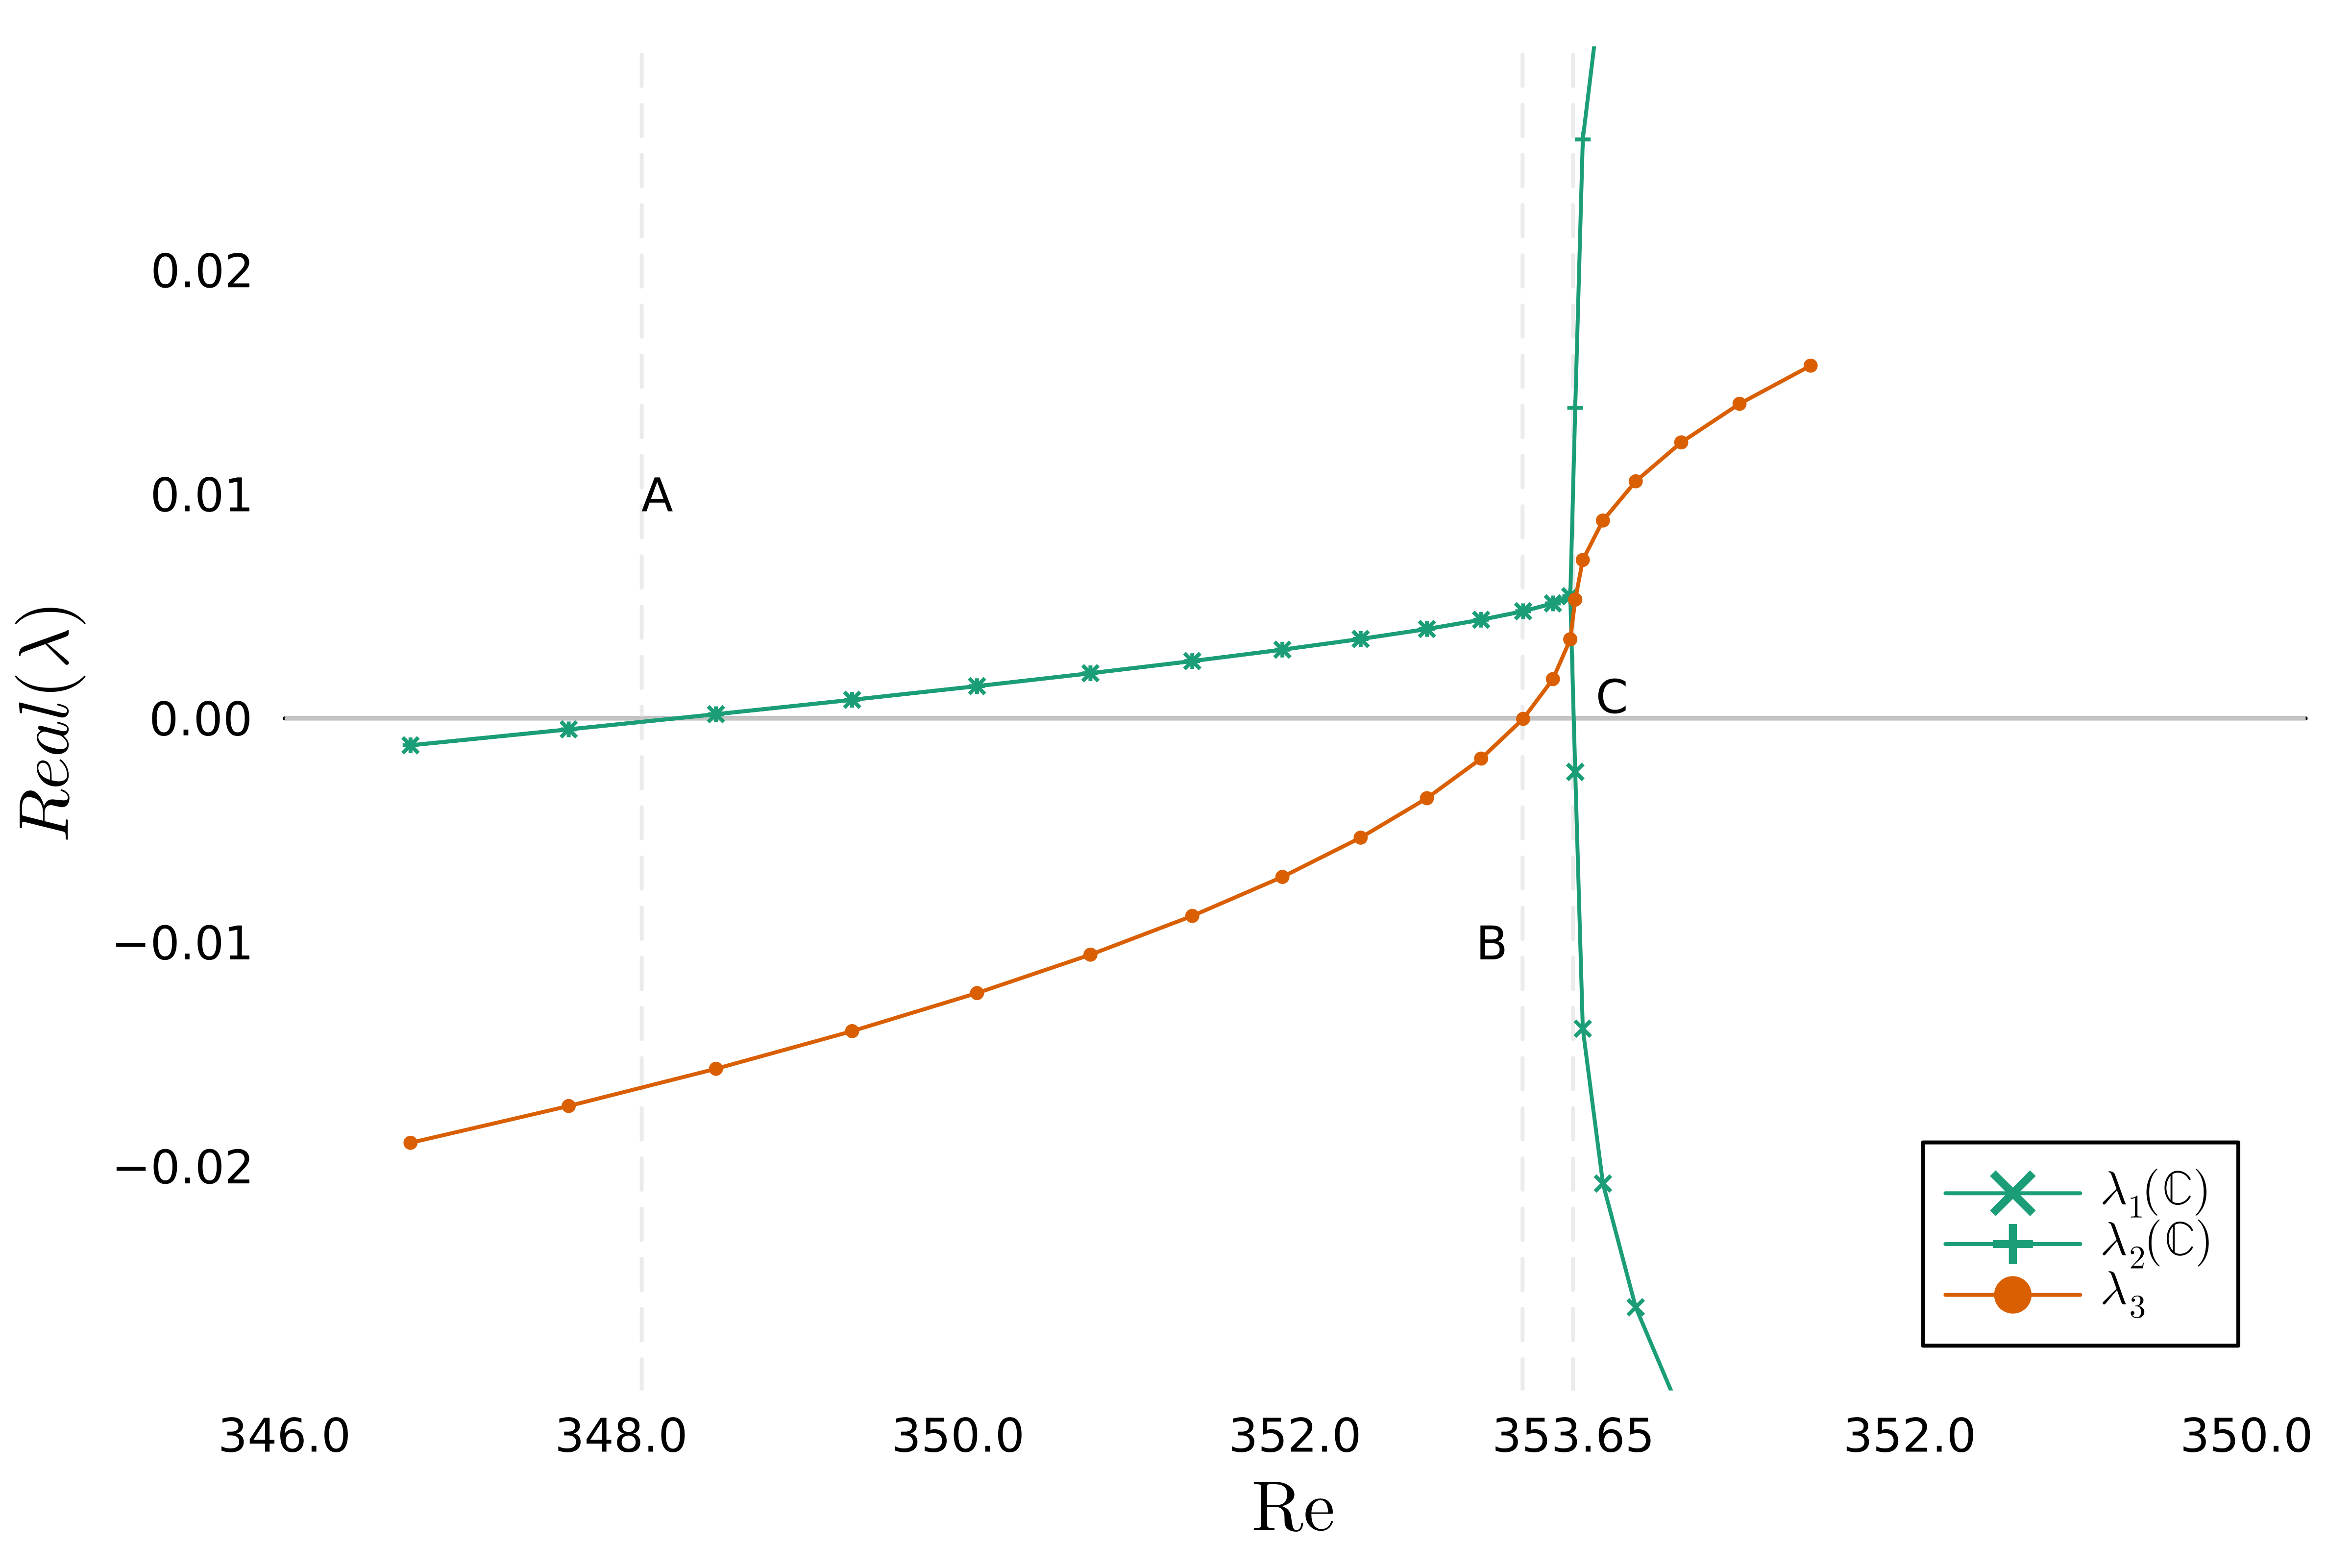
\includegraphics[width=0.6*\textwidth]{figs/lsa_sn}
  \end{center}
  \label{fig:lsa}
  \caption{Linear stability analysis around saddle node (increasing and the decreasing Renolds number). The real
    part of the largest eigenvalues are plotted} 
\end{figure}

Close to the saddle node there is another branch appearing this branch is. This
can be detected by starting natural continuation algorithm close to branch. It
is not yet clear what actually happens there but the simplest explanation being
that at the first crossing B in figure \ref{fig:lsa} corresponds to the
emergence of this new branch. But a linear stability analysis around shows that
the linear stability analysis around the saddle node shows that the complex
conjugate pair seems to be 0 at this precise location. Below the values at the
center of the streamfunction are compared for the different eigenvalue crossing.



\subsection{Further work}

There multiple things going on around. To get clear picture one could change
velocities and A further thing to be done is computing the bifurcation. 




This problem was chosen with the primary intention to investigate this
benchmark and test Navier-Stokes on t 


Lastly it has to be mentioned that there is










This problem was chosen with the primary intention to investigate this
benchmark and test Navier-Stokes on t 





